\chapter{Gestion du projet}
\section{Organisation du projet}
Dès le départ, nous avons décider de travailler avec git, plus précisement 
sur \href{https://github.com}{github}. Nous avons donc créé une organisation afin de séparer les différents dépots. Nous en avons définis 2, mais les membres de l'organisation étaient libres d'en ajouté d'autres.
\begin{itemize}
    \item crapauduc.  Ce dépôt est le dépot principal où les notebooks des modèles sont déposés, nous y avons aussi placé les rapports des anciens étudiants afin d'y avoir un accès rapide. Nous y avons aussi déposé unun subset d'image d'environ 0.5 Gib permettant le fine tuning.
    \item utils. Ce dépôt contient des scripts faisant des transformormations ou des analyses sur les données. Nous y avons par exemple un script qui permet de convertir les annotations de csv à COCO.
\end{itemize}

De plus, nous avons créer un compte google ayant le doux nom de \verb|student GML| afin d'avoir un espace google drive de 15 GiB pour stocker les données ainsi qu'une intégration facilitée dans le service \href{https://colab.research.google.com/}{colab} de Google. Nous croyions être prêts.


\section{Gestion du temps de travail}
Dès le départ, nous avons décider de travailler à distance afin de dédier 
la totalité de la journée à ce projet sans perdre de temps dans les transports publiques. En effet, le mardi où tombe le cours de GML, nous n'avons pas d'autre cours que ce dernier. Ainsi, un mardi typique se déroule comme suit:
\begin{itemize}
    \item 8h00 - 13h15: Libre, mais souvent on prépare la séance de l'après-midi.
    \item 13h15 - 15h: Appel Teams, où nous expliquons notre avancement, normalement les différents problèmes rencontré doivent être réglé avant la réunion. Planification des tâches pour la prochaine semaine, et répartition des tâches. Durant chaque réunion un membre du groupe prend des notes afin d'avoir un historique des discussions, ce procès verbale des réunions est stocké sur le google drive de \verb|student GML|.
    \label{item:seance}
\end{itemize}
La séance du mardi se résume donc essentiellement à un partage d'information entre les différents groupes de travail composé de 1 à 3 étudiant.e.s. Le travail proprement dit est pour la plupart effectué en dehors des réunions, soit le mardi après la réunion soit à un autre moment choisis par les membres du groupe.

\section{Gestion des tâches et répartition}
Nous avons poussé notre utilisation de \href{https://github.com}{github}, en gérant nos tâches à l'aide de l'outil de gestion de projet \href{https://github.com/topics/kanban}{kanban} directement intégré dans \href{https://github.com}{github}. Ainsi, nous pouvons savoir à n'importe quel moment quel membre de l'équipe travail sur quelle partie du projet. De plus, nous pouvons voir les tâches en cours, les tâches terminées, les tâches en attentes, etc. 

\begin{figure}[htb!]
    \centering
    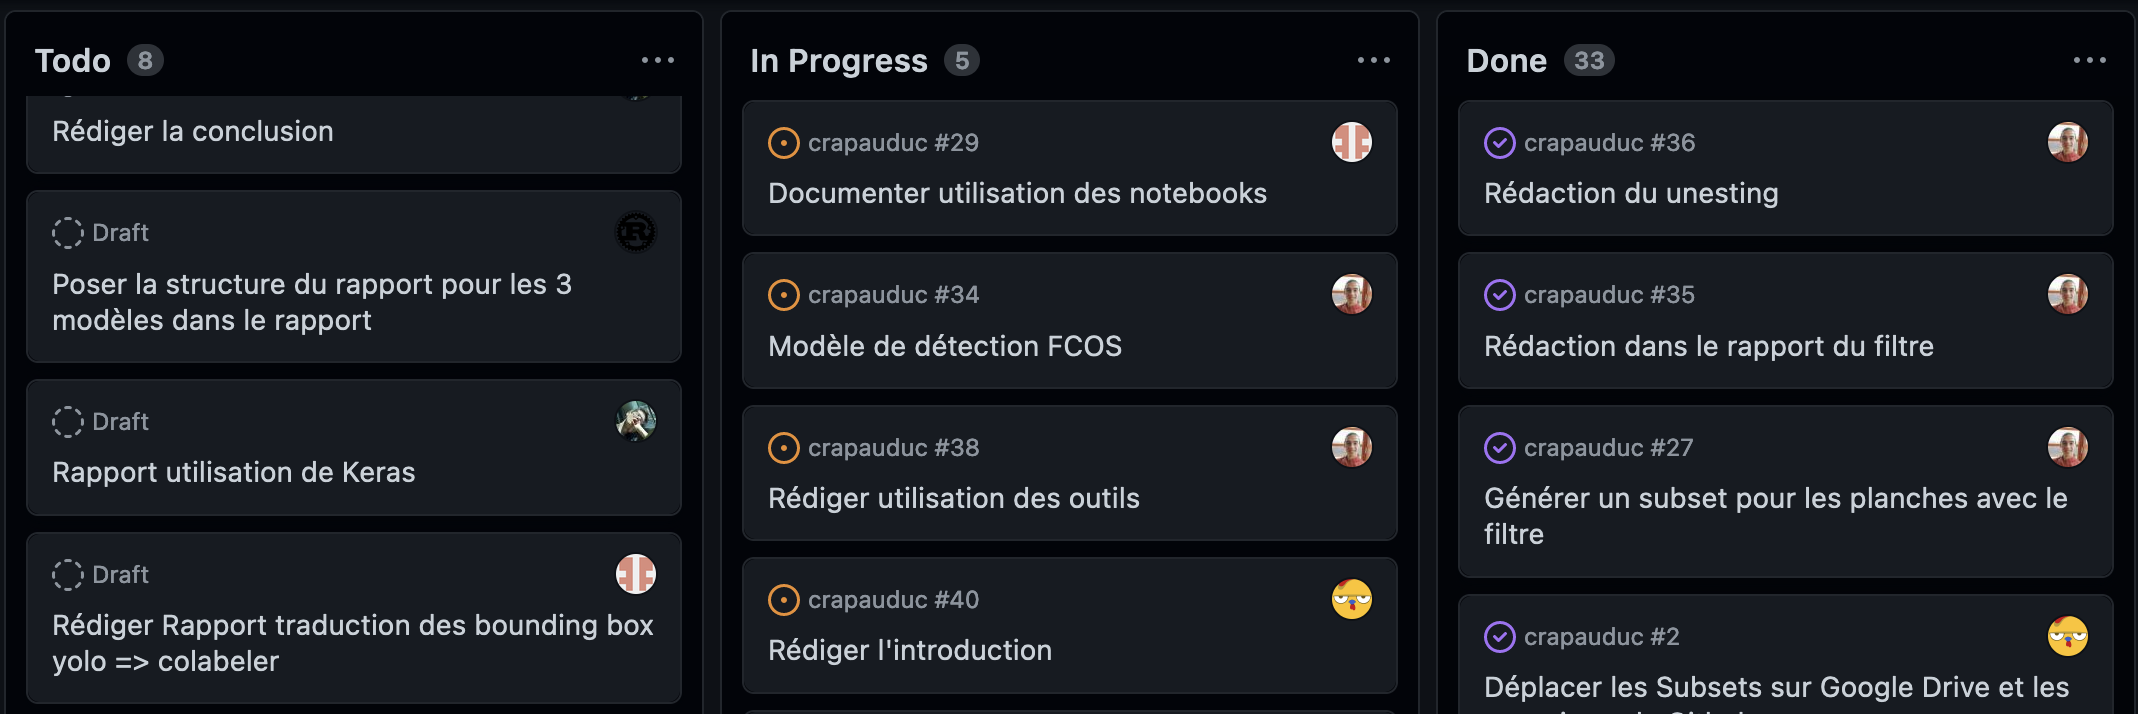
\includegraphics[width=0.8\linewidth]{images/kanban.png}
    \caption{Nos tâches du Kanban réparties en 3 catégories : à faire, en cours et terminées.}
    \label{fig:kanban}
\end{figure}
